\documentclass{article}
% Chinese
% \documentclass[UTF8, nofonts, mathptmx, 12pt, onecolumn]{article}
% \usepackage{xeCJK}
% \setCJKmainfont{SimSun}
\usepackage{amsmath}
\usepackage{amsfonts}
\usepackage{amssymb}
\usepackage{wasysym}
% \usepackage{ctex}
\usepackage{graphicx}
\usepackage{float}
\usepackage{geometry}
\geometry{a4paper,scale=0.8}
\usepackage{caption}
\usepackage{subcaption}
% \newcommand{\oiint}{\mathop{{\int\!\!\!\!\!\int}\mkern-21mu \bigcirc} {}}
\newcommand*{\dif}{\mathop{}\!\mathrm{d}}
\newcommand*{\md}{\mathop{}\!\mathrm{d}}
\newcommand*{\me}{\mathrm{e}}

% \usepackage{parskip}
% \setlength{\parindent}{0cm}

\usepackage{bm}
\let\Oldmathbf\mathbf
\renewcommand{\mathbf}[1]{\boldsymbol{\Oldmathbf{#1}}}
\let\eqnarray\align

\author{Xiping Hu}
\usepackage{authblk}
\author{Xiping Hu}
\affil{http://thehxp.tech/}
\title{Homework for Chapter 3}

\begin{document}
\maketitle

\begin{figure}[H]
  \centering
  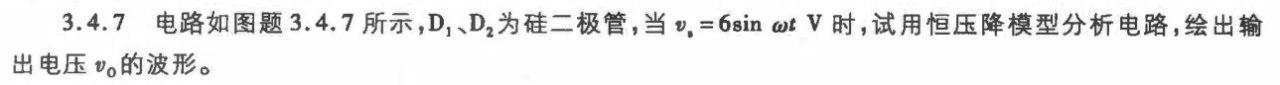
\includegraphics[width=\linewidth]{figures/Problem1-1}
  \label{fig:}
\end{figure}
\begin{figure}[H]
  \centering
  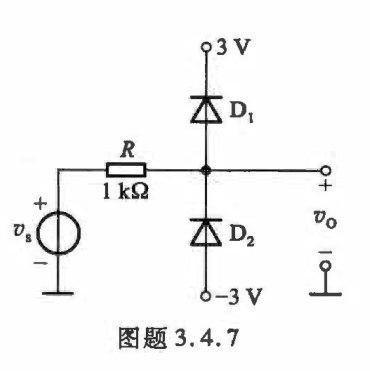
\includegraphics[width=0.7\linewidth]{figures/Problem1-2}
  \label{fig:}
\end{figure}

From the circuit we shall know, if the forward voltage of the 2 dipoles are $0.7 \  \mathrm{V}$:
\begin{itemize}
\item A current flows in $D_1$ whenever $v_s > 3.7 \  \mathrm{V}$
\item A current flows in $D_2$ whenever $v_s < - 3.7 \  \mathrm{V}$
\end{itemize}

So that the voltage is being restricted between $\pm 3.7 \  \mathrm{V}$ 


\begin{figure}[H]
  \centering
  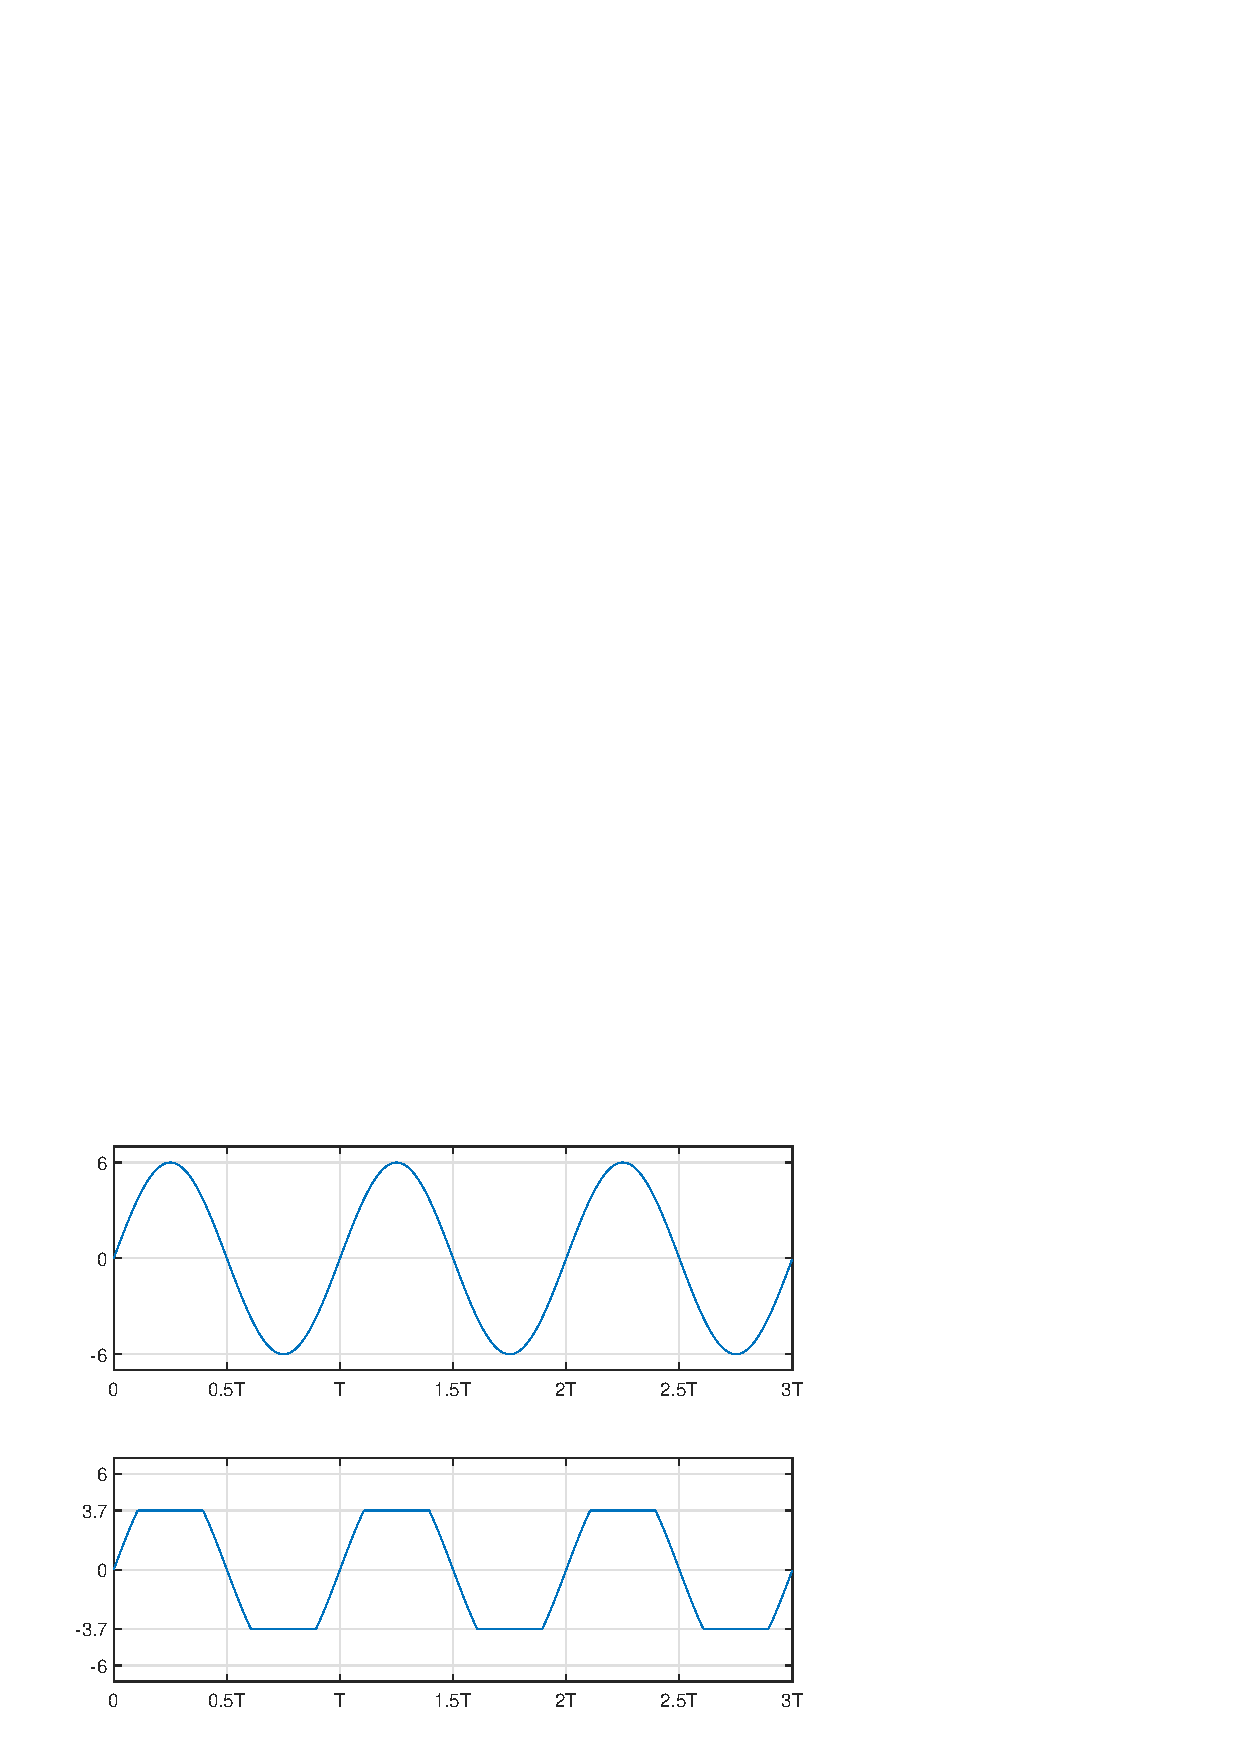
\includegraphics[width=\linewidth]{figures/Problem1-3}
  \label{fig:}
\end{figure}


\end{document}